\documentclass[a4paper]{article}

\usepackage{amsmath, graphicx, float, blindtext} % for dummy text
\graphicspath{ {./images/} }
\title{Goals, Power and Sample size}
\author{Shubham Gupta}

\begin{document}
\maketitle
\section{Introduction}
\begin{itemize}
    \item Statistical methods allow us to measure the \textit{probability} of achieveing a goal \textit{given that} the underlying assumptions are true.
    \item All experiment goals can be expressed in the form of HDI's.
\end{itemize}
\subsection{Power}
\begin{itemize}
    \item Probability of acheiving goal, given hypothetical state of the world and the sampling process, is the \textbf{power} of planned research. 
    \item Method to increase chance of detecting an effect: 
        \begin{itemize}
            \item Reduce measurement noise.
            \item Amplify magnitude of underlying effect.
            \item Increase sample size. Sample size increases $\implies$ Power increases. 
        \end{itemize}
    \item We will repeating sample from datasets that contain points we expect to see, and perform Bayesian analysis on them before performing the actual experiments. A "dress rehearsal" of sorts.
        \begin{figure}[H]
            \centering
            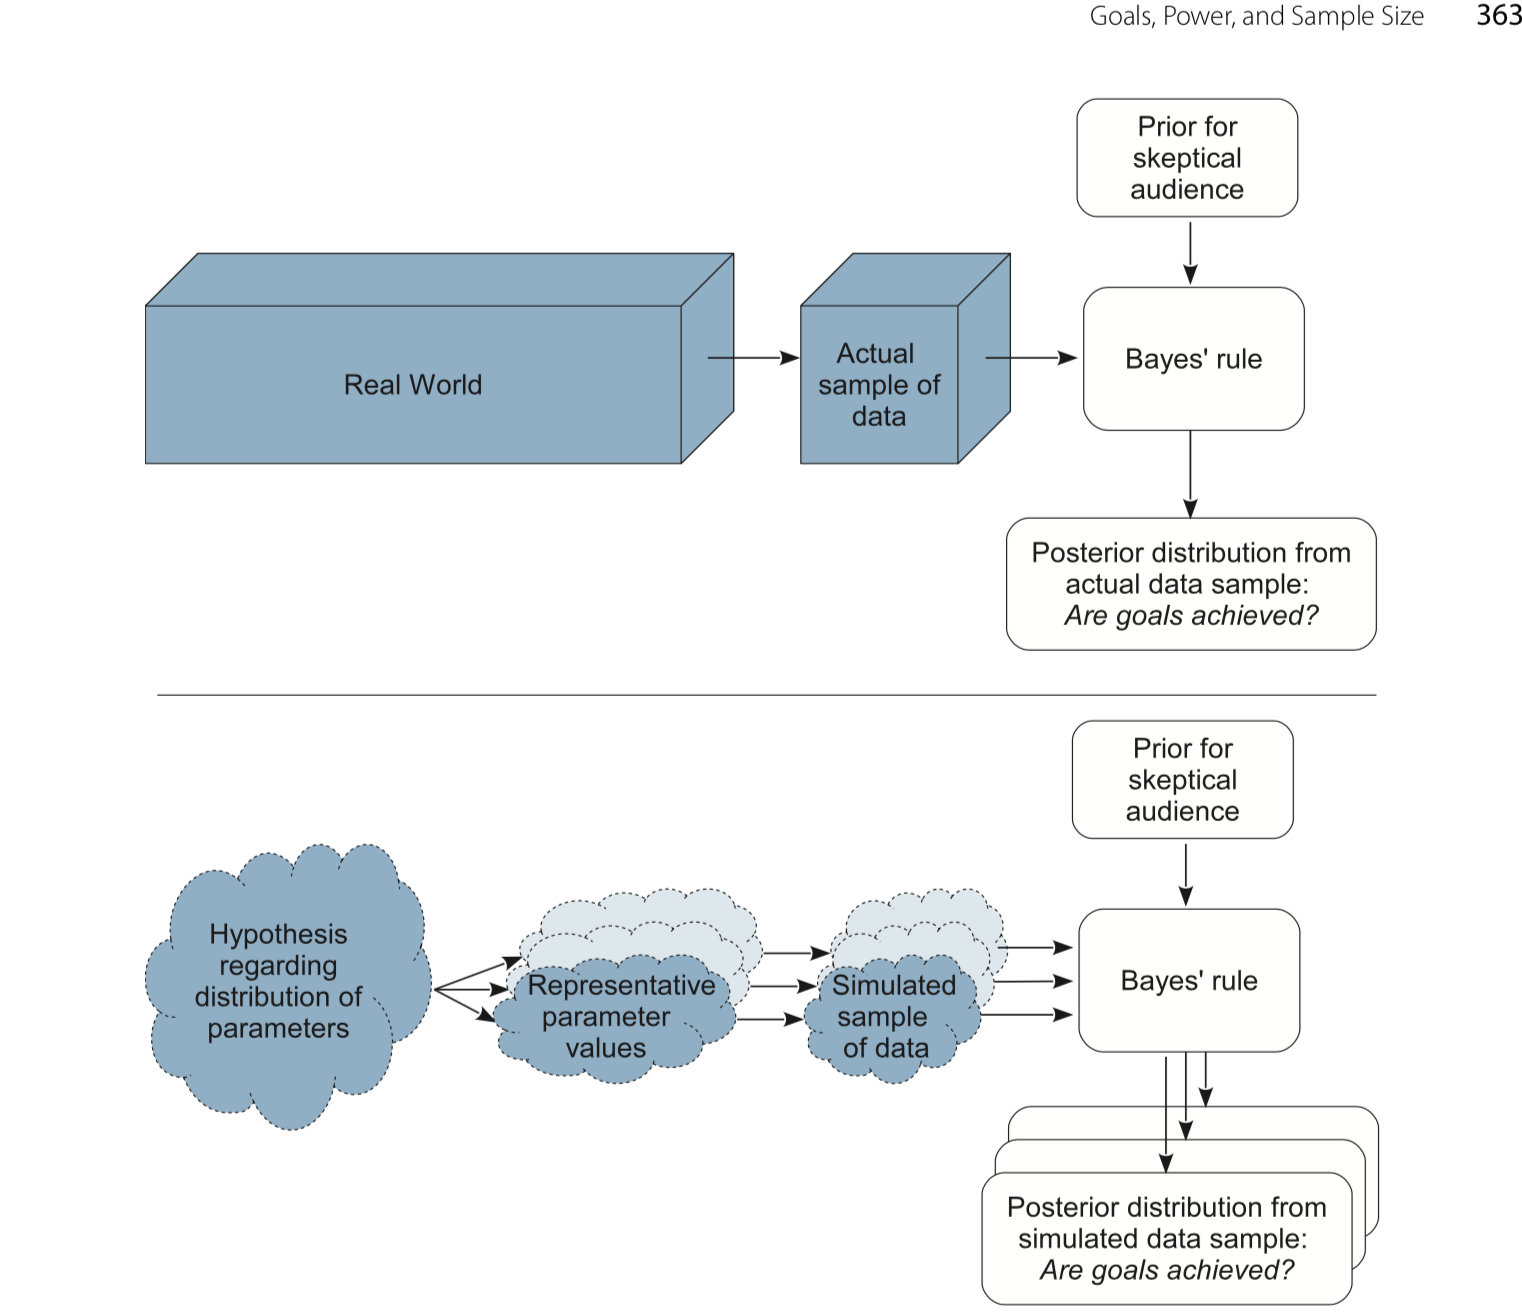
\includegraphics[width=0.8\textwidth]{real_world_vs_power_analysis}
            \caption{Real world vs Power analysis}
            \label{fig:real_world_vs_power_analysis}
        \end{figure}
    \item For power analysis, we do the following:
        \begin{itemize}
            \item From hypothetical distribution of values, generate representative values.
            \item From representative values, generate random sample of data, using a planned sampling method. The sampling method should be the \textbf{same} as expected to be used in the real world experiment. 
            \item From random sample, compute posterior using Bayesian analysis and appropriate priors.
            \item From posterior estimate, check if the goals were acheived or not.
            \item Repeat the process many times to increase the power.
        \end{itemize}
\end{itemize}
\subsection{Sample Size}
\begin{itemize}
    \item Large sample sizes will help make the posterior distribution narrower thereby giving us more confidence in our results. 
    \item If we are trying to prove that a value is different from the null hypothesis, \textbf{sometimes} large samples will not be enough. They will just show how the \textbf{sampling process} was performed.  
    \item For eg, if we think a coin is baised, and the changes of the theta value assigned as: $ p(\theta = 0.5)=0.25 , p(\theta =0.7) =0.25, p(\theta=0.8) =0.50 $, then even with a large amount of data, the maximum probability we can get that discards the  $p(\theta=0.5)$ null hypothesis is $0.75$.
\end{itemize}
\subsection{Other expressions of goals}
\begin{itemize}
    \item Average width of HDI over different trails should excede a value L.
    \item It can also be measured using \textbf{entropy}. The goal will be to have a low entropy.  
    \item Goal can also be to obtain a sufficiently large Bayes factor.
\end{itemize}
\section{Computing Power and Sample Size}
\begin{itemize}
    \item We will go through the above process to find exact number of samples needed for various degrees of power for different data-generating hypothesis.
\end{itemize}
\subsection{Goal is to exclude null value}
\begin{itemize}
    \item If aim is to exclude null value, we must prove that HDI does not include ROPE for that null value.
    \item We need to geenrate a parameter distribution which will be used to generate data.
    \item \textbf{Simple method}: Use posterior distribution obtained from data and prior(could be actual or expected) as parameter distribution. This approach is called as \textbf{equivalent prior sample} method. 
    \item Once we have the hypothetical distribution, we sample from it to get a representative parameter value. Using this value, we generate a data point.
    \item The process looks as follows:
        \begin{itemize}
            \item Select a value for the \textbf{true} bias of the coin, centered around your hypothesis(in this case, around $\theta = 0.65$. 
            \item Simulate flipping a coin with this bias \textbf{N} times. With \textbf{z} heads, proportion of heads will be $ \frac{z}{N}$. 
            \item Using audience appropriate priors(not sure what this means), determine posterior beliefs about $\theta$. Check if ROPE excludes $\theta=0.5$. 
            \item Repeat this process many times to determine power.
                \begin{figure}[H]
                    \centering
                    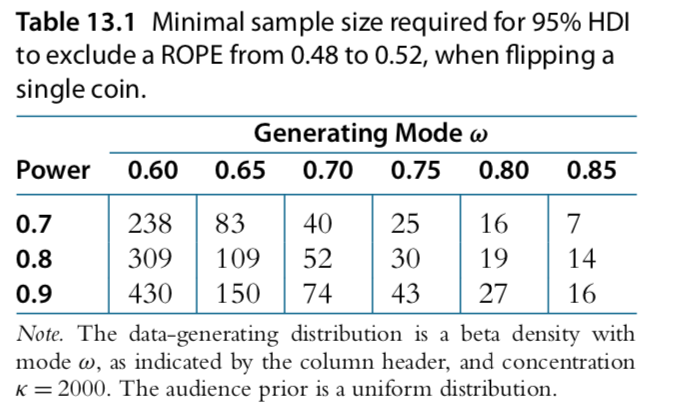
\includegraphics[width=0.8\textwidth]{power_table}
                    \caption{Power table}
                    \label{fig:power_table}
                \end{figure}
            \item The table above shows how the sample size varies with the mode. When the mode is large, the sample size is small. This makes sense \textbf{because} large mode $\implies$ higher proportion of heads $\implies$ $\theta$ HDI falls well above 0.5
            \item When the mode is only slightly above 0.5, then it will take a large number of samples for the HDI to \textbf{consistently} fall ourside the ROPE of 0.5.
            \item Increase in power $\implies$ Increase in the number of samples needed.
        \end{itemize}
\end{itemize}

\subsection{Goal is precision}
\begin{itemize}
    \item If we need to determine which variant of A or B is more preferred, how many samples would we need to show that 80\% of the time 95\% HDI falls about $\theta=0.5$?
    \item Problems: When \textbf{N} is large, HDI will be around the intial $\theta$ value used. 
    \item Instead of proving intial $\theta$ value lies outside the HDI, we will try to show width $L$ of the HDI is always less than a value, say 0.2. Less width $\implies$ Narrow HDI $\implies$ Higher confidence on posterior values.
    \begin{figure}[H]
        \centering
        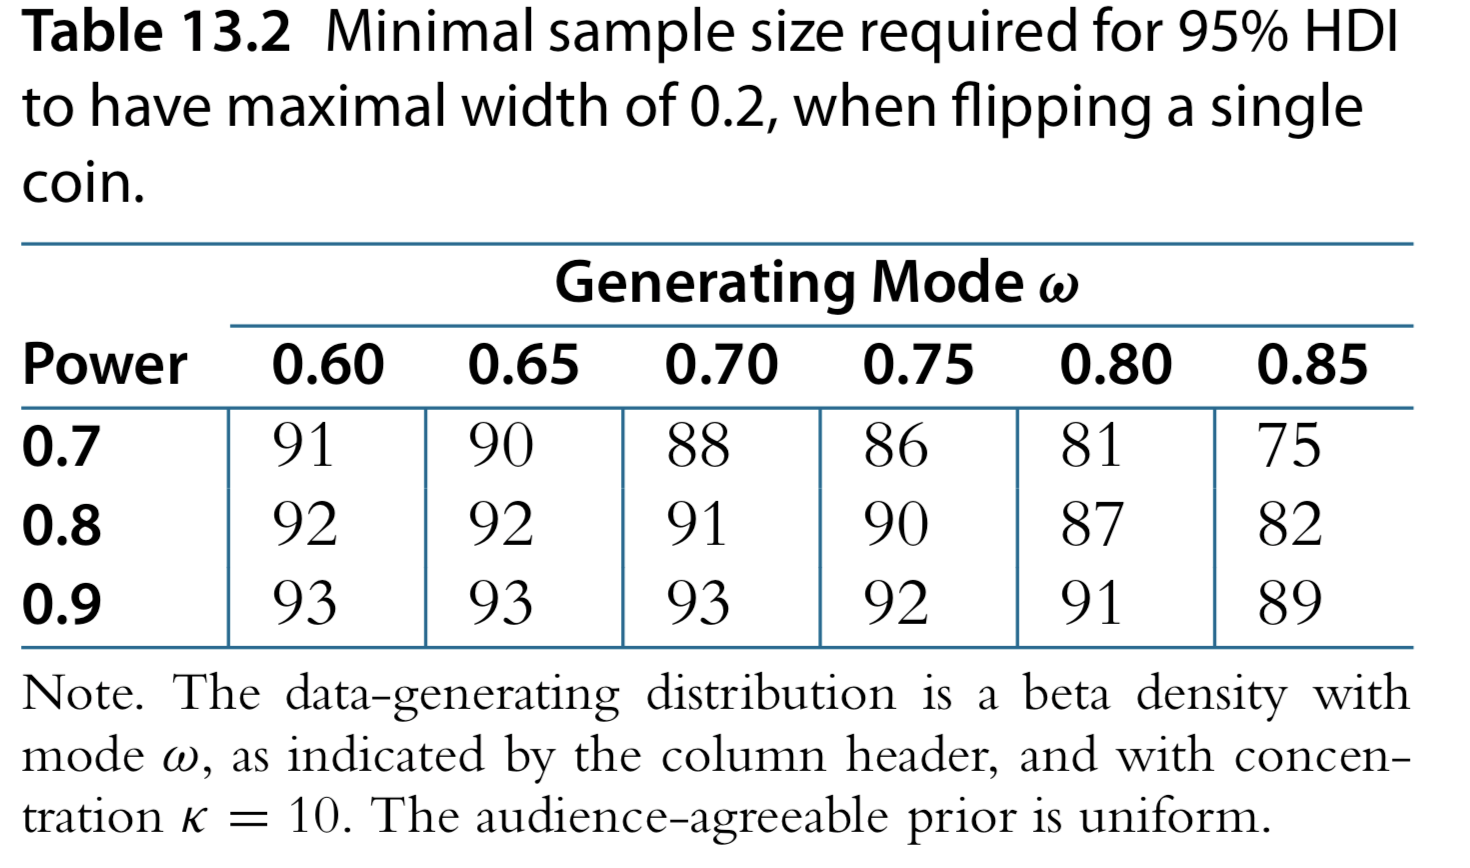
\includegraphics[width=0.8\textwidth]{width_power_table}
        \caption{Power table for width of HDI}
        \label{fig:}
    \end{figure}
    \item Increase in power only has \textbf{marginal increase} in sample size. This is because distribution of HDI widths has shunted high tail. Small changes in $N$ can pull high tail towards threshold values like 0.2. 
    \item HDI width decrease $\implies$ $N increases$ rapidly. 
\end{itemize}

\subsection{Monte Carlo approximation of power}
\begin{itemize}
    \item Script present to do power calculations of complex models. Will all more details when I'm implementing it.
\end{itemize}
\subsection{Power from idealized or actual data}
\begin{itemize}
    \item Use actual/\textit{hypothesized} data to represent top level paramters.
    \begin{figure}[H]
        \centering
        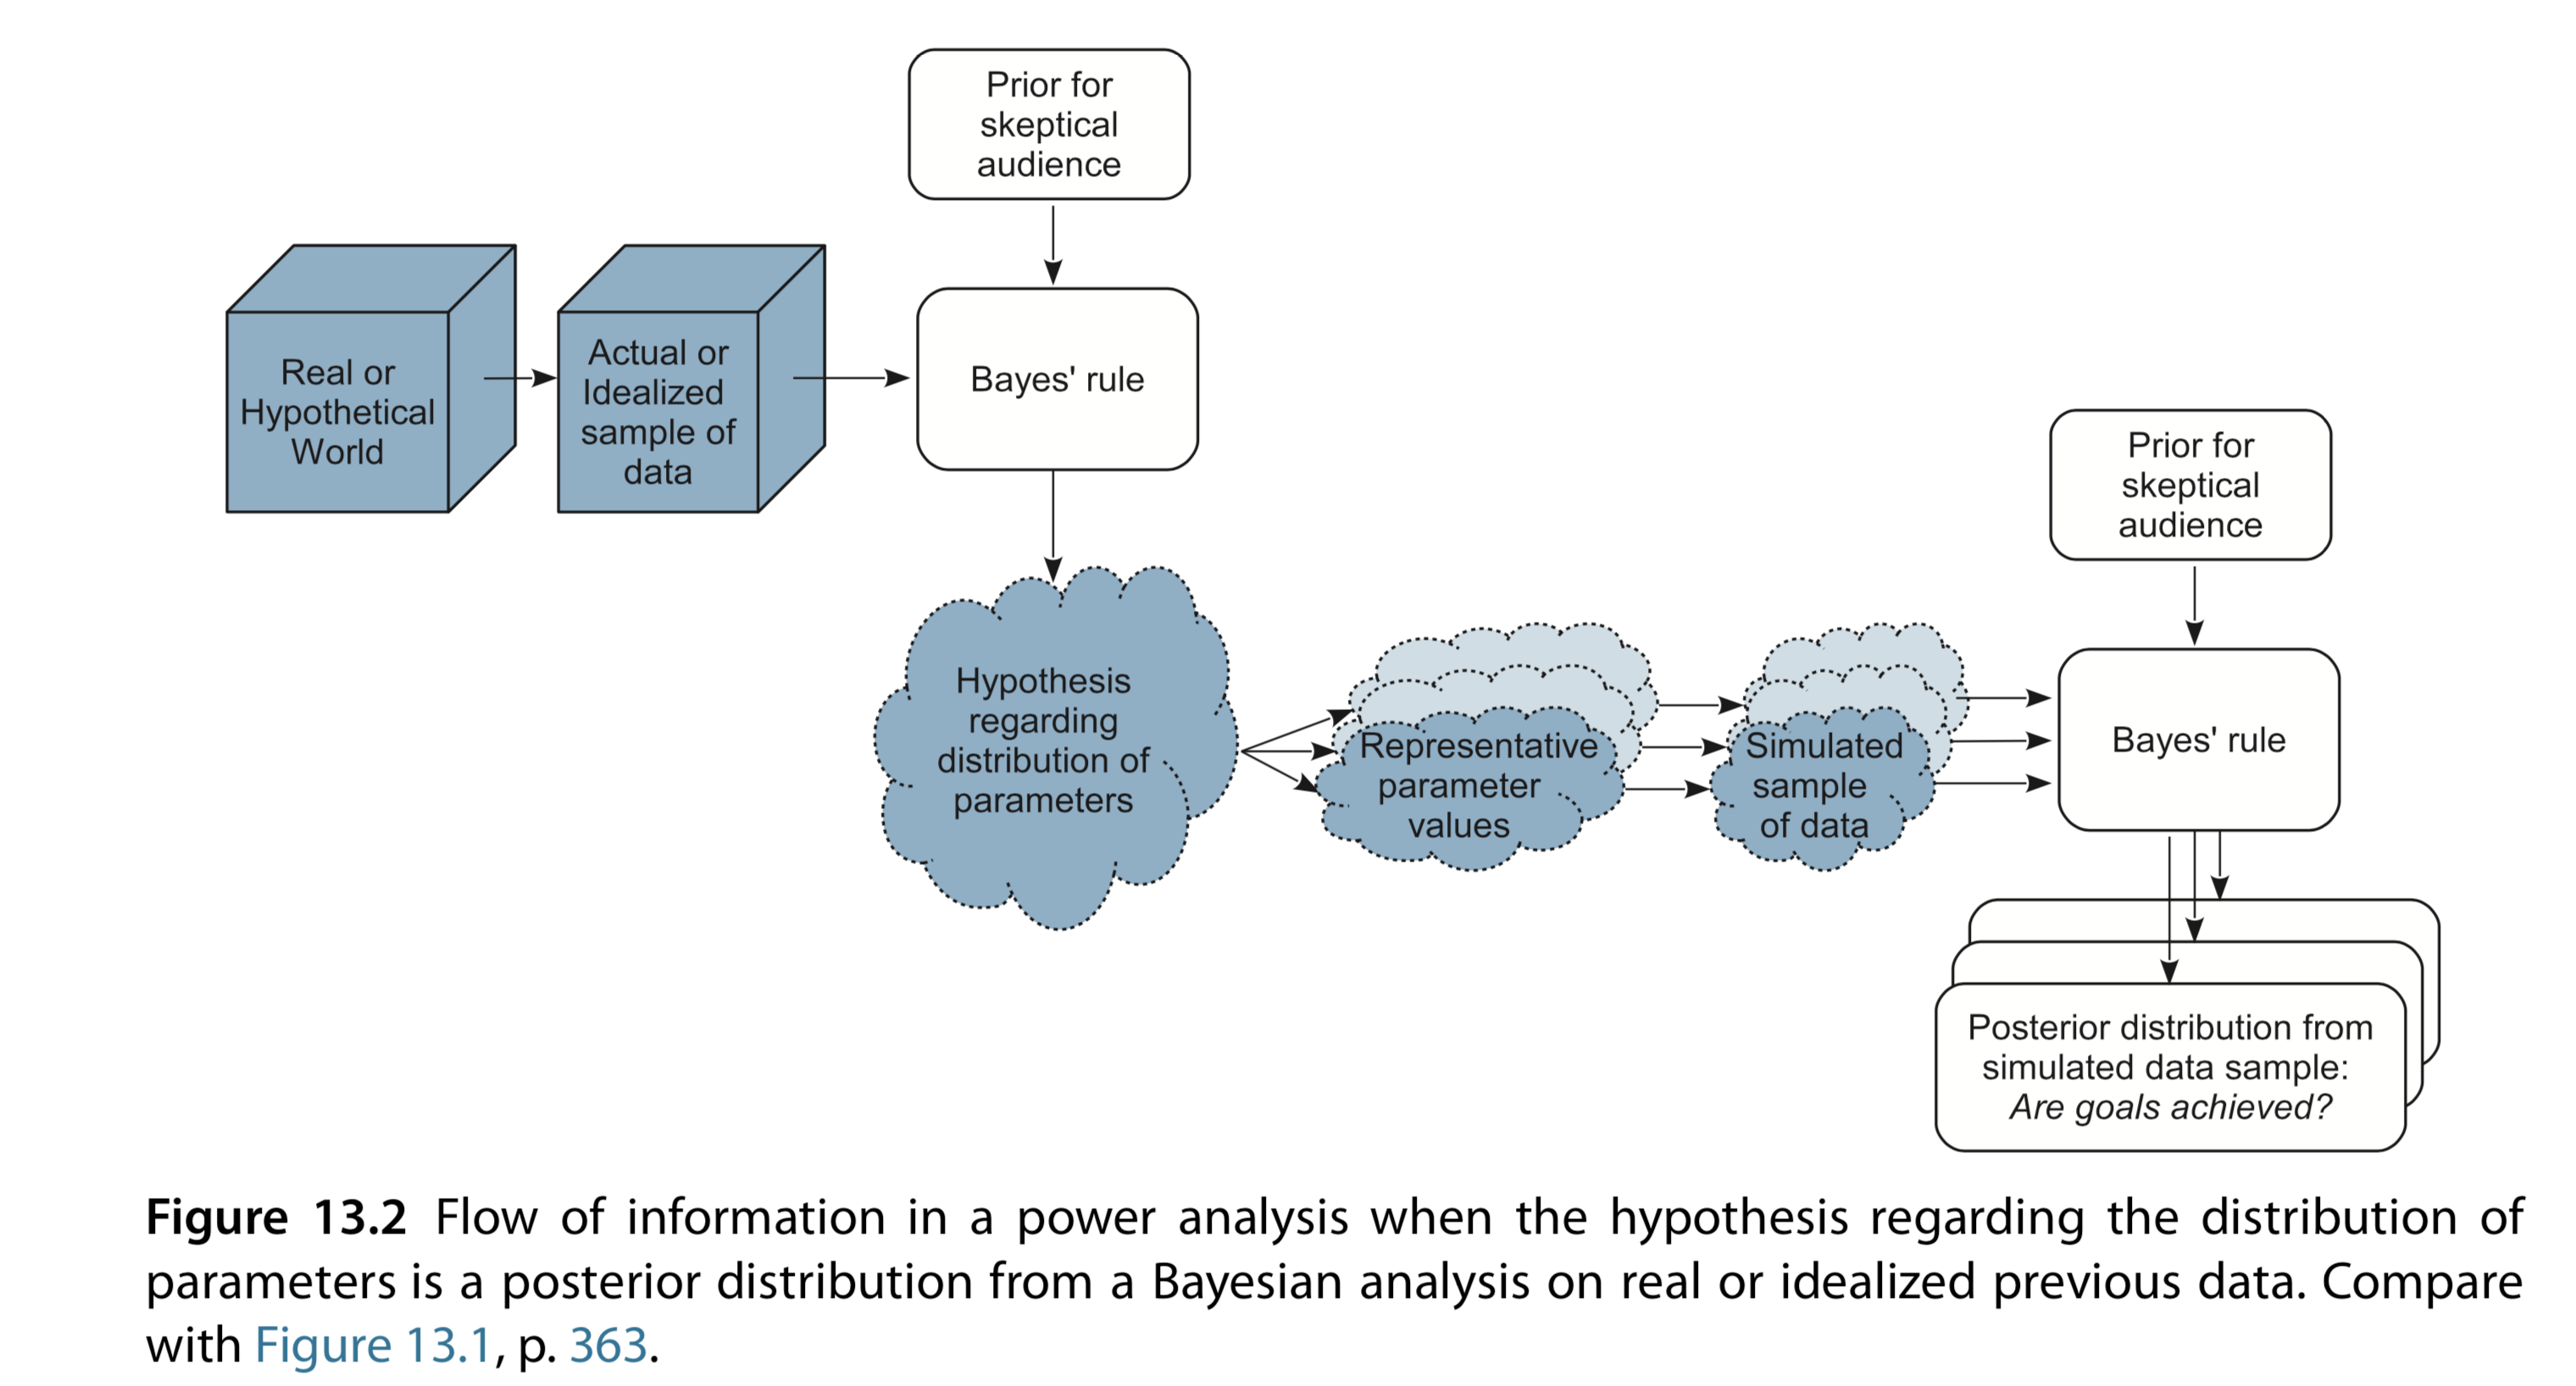
\includegraphics[width=0.8\textwidth]{info_flow_power}
        \caption{Information flow for power analysis}
        \label{fig:info_flow_power}
    \end{figure}
    \item Benefits of using this approach:
    \begin{enumerate}
        \item Hypothesis is expressed as easily understandable data and bayesian analysis will convert it into parameter distributions.
        \item Corelation between the parameters are automatically created in the posterior distribution
    \end{enumerate}
    \item Long example around how to do power analysis. This will be implemented in the code.
\end{itemize}
\section{Sequential testing and goal of precision}
\begin{itemize}
    \item Comparison between bayesian method and NHST. Basically claims that practice of always rejecting null hypothesis is not correct.
    \item Instead of rejecting null hypothesis, we should aim for precision. This is because precision for most parameters is unaffected by the true underlying value of the parameter.
    \item We will compare the appraoches of p-values, Bayes Factors(BF), HDI with ROPE and precision(width of HDI interval).
\end{itemize}
\end{document}
